
\NeedsTeXFormat{LaTeX2e}
\documentclass[12pt]{article}

\usepackage{titlesec}
\usepackage{setspace}
\usepackage{amsmath}
\usepackage{amssymb}
\usepackage{epsfig}
\usepackage{fancybox}
\usepackage{listings}
%\usepackage{algo}
\usepackage{url}
\usepackage{xcolor}
\usepackage{adjustbox}
\usepackage{float}
\usepackage{multicol}
\usepackage[utf8]{inputenc}
\usepackage[colorlinks=true,linkcolor=blue]{hyperref}

\newcommand{\phil}[1]{{\color{red}(\textbf{Phil:} #1)}}
\newcommand{\yue}[1]{{\color{blue}(\textbf{Yue:} #1)}}
\newcommand{\specialcell}[2][c]{%
	\begin{tabular}[#1]{@{}c@{}}#2\end{tabular}}


\setlength{\textheight}{9in}
\setlength{\textwidth}{6in}
\setlength{\oddsidemargin}{.25in}
\setlength{\topmargin}{-.5in}  % changed from -.25 by RSR on 1/21/07
%\parindent .5in    % commented out by RSR 1/21/07

\hyphenation{itself}
\setcounter{secnumdepth}{4}
\setcounter{tocdepth}{4}
%%%%%
%% Commented out -- RSR, 1/21/07
%%%%%
% The following provides a box to surround the thesis statement
\newenvironment{Thesis}%
{\begin{Sbox}\begin{minipage}{.95\linewidth}}%
		{\end{minipage}\end{Sbox}\begin{center}\fbox{\TheSbox}\end{center}}

\title{Stream Mining Algorithms for Sensor Data Classification}
\author{
	Yue Dong\\
	\texttt{yuedong029@uottawa.ca}
	\and
	Philippe Paradis\\
	\texttt{philippe.paradis@carleton.ca}
}

\begin{document}

	\singlespace
	\maketitle
	
	\tableofcontents
	\newpage
	\section*{Acknowledgements}
	
	
	\begin{abstract}                % ~350 words max
		
		
	\end{abstract}
	
	% This sets section-numbering to only include Section and Subsection numbers
	\setcounter{secnumdepth}{4}
	
	\section{Introduction}
	\label{sec:introduction}

        Bicycle sharing systems have seen have seen a surge in popularity throughout the world since the mid-2000s. For example, Bixi was launched in 2008 in Montreal and is now the largest bike sharing system in Canada. It was quickly followed by Capital Bixi in Ottawa/Gatineau in June 2009. There are now more than 700 cities worldwide with bicycle sharing systems! Part of the reason for the sudden large-scale adoption of those systems is the advance in technology, lowering initial costs and increasing profit margins for companies. Most important of all, advances in information technology significantly improved the viability of this type of business. Modern technology allows companies to automate bike rentals, drop-offs, reservations and fleet tracking. It also makes it more convenient to the user and deters theft by requiring large credit card deposits. Bla bla.

Since bike sharing systems are all automated, tons of very detailed data has been collected about the usage of those systems.

In particular, many organisations operating bike sharing systems are public organisations, such as cities, or private-public partnerships. As a consequence, those organisations tend to frequently make part of their data available to the public!

Part of the reason for the success and 
        In this project, we investigate a modern dataset rel the usage of city bike sharing systems
	
	Philippe's introduction draft:
	\begin{enumerate}
		\item Load data
		\item Basic data pre-processing
		\item Imputation (Numeric variables, categorical variables, analysis)
		\item Visualization (most of it Yue is in charge, but I performed visualization of imputations as well as visualization for the each day in the entire 2 years's worth of data for casual, registered and cnt...)
		\item Data augmentation: add previous X hours as columns... for example, add "cnt.1hrago", ..., "cnt.24hrago" (work in progress)
		\item Features Engineering:
		\begin{itemize}
			\item Added a "bad rows" column, where rows with poor imputation results are flagged and discarded from the training phase)
			\item Added "special events", such as Christmas, where we expect lower demand for bike rental
			\item Designated some non-holiday days as being holidays anyway. For example, whenever a Thursday is a holiday, then the Friday right after it will be designated a holiday too. Whenever a Tuesday is a holiday, then the Monday right before it will be designated as a holiday too.
			\item Transform \texttt{atemp} into \texttt{atempdiff} (i.e. the distance between the current apparent temperature and the ``ideal'' apparent temperature)
			\item Transform \texttt{hum} into \texttt{humdiff} (similar idea)
			item Auxiliary datasets (work in progress...)
		\end{itemize}
		\item Did my own version of association rules mining, including using the hyperlift measure (found nothing interesting)
		\item Supervised learning:
		\begin{itemize}
			\item Built a Random Forest classifier (fast, average results)
			\item Built a neural network classifier using \texttt{nnet} (moderately slow, good results)
			\item Used the following features:
			\begin{verbatim}
			c("season","yr","mnth","hr","weekday","workingday",
			"weathersit","atempdiff","hum","windspeed")
			\end{itemize}
			\end{verbatim}
			\item Performed a grid search to find ideal parameter of neural network
			\item Ranked in the top 150 on Kaggle
			\item Noticed that my model tended to overfit and that better scores would frequently be obtained when using very small number of epochs
			\item Switched to \texttt{avNNet}, a parallel ensemble method for neural network
			\item Speed remained the same, results improved considerably
			\item Rank position on Kaggle yet to be determined
			\item Attempted a Deep Neural Network model with the package \texttt{h2o}. The package is incredibly fast and very easy to interface with, unfortunately I found the neural network model to be extremely unstable. I could not obtain better results than with the simpler single-hidden layer neural networks above.
			\item Attempted to use the \texttt{RSNNS} package to train a Jordan neural network, which is a type of recurrent neural network designed specifically to perform well with time series. Unfortunately, the package would always crash R and I never managed to get it to work.
		\end{itemize}
	\end{enumerate}
	
	\subsection{Questions}
		What relationships do we expect to see in the data?
		\begin{itemize}
			\item Variation in bike rentals based on hour of the day
			\item Different bike rental patterns on the weekends versus regular weekdays
			\item Different  bike rental patterns on holidays versus non-holidays
			\item Variation in bike rentals based on temperature
			\item Variation in bike rentals based on weather condition
			\item No idea about effects of humidity
			\item Variation in bike rentals based on wind speed
		\end{itemize}
		
		What kind of relationships do we expect to see in the data?
		\begin{itemize}
			\item On regular weekdays, spike in traffic during morning and afternoon rush hours
			\item Typically, higher bike rental volumes during the day and lower during the night
			\item In other words, highly non-linear relationship between bike rentals and datetime
			\item Roughly linear variation between bike rentals and temperature (although very high summer temperatures could lead to reduced bike rental volumes)
			\item 
		\end{itemize}
		
		%\subsection{Missing values}
		
		- What could possibly explains the missing values that we see?
		There is clearly a pattern in the missing values. Most of those happen at the same time at night.
		Also, the bike count values tend to change and be much smaller around missing values. Why is that?
		
	
	\section{Dataset \& Data exploration}
	\subsection{Dataset}
	The dataset we used is the Bike Sharing Dataset from the UCI repository. According to the dataset description, ``this dataset contains the hourly and daily count of rental bikes between years 2011 and 2012 in Capital bikeshare system with the corresponding weather and seasonal information.''
	The summary of this dataset is as Table \ref{table:dataset} shows. More information of the dataset can be found at \url{http://archive.ics.uci.edu/ml/datasets/Bike+Sharing+Dataset}.
	
	\begin{table}[H]
		\begin{tabular}{| p{5cm} | p{11cm} |} \hline
			Number of instances: & 17389 (hourly), 731 (daily)\\
			Number of Attributes: & 16\\ 
			Attribute Characteristics: &  Categorical, Integer,
			Date/time, Decimal\\
			\hline \hline
			\textbf{Attributes Information:} &\\ \hline
			\textbf{Attribute name } & \textbf{Description}\\ \hline
			instant   & record index\\ \hline
			dteday    & date\\ \hline
			season   & season (1:springer, 2:summer, 3:fall, 4:winter)\\ \hline
			yr    &  year (0: 2011, 1:2012)\\ \hline
			mnth &   month (1 to 12)\\ \hline
			hr & hour (0 to 23) \\ \hline
			holiday   & whether day is holiday or not \\ \hline
			weekday   &  day of the week \\ \hline
			workingday   & 1: if day is neither weekend nor holiday; 0: otherwise.\\ \hline
			weathersit   & 1: Clear; 2: Mist; 3: Light Snow, Light Rain; 4: Heavy Rain, Ice Pallets, Snow + Fog;\\ \hline
			temp   & Normalized temperature in Celsius \\ \hline
			atemp    & Normalized feeling temperature in Celsius \\ \hline
			windspeed   & Normalized wind speed \\ \hline
			casual   & count of casual users\\ \hline
			registered   & count of registered users\\ \hline
			cnt   & count of total rental bikes including both casual and registered \\ \hline
		\end{tabular}
		\caption{Summary of the bike sharing dataset}
			\label{table:dataset}
	\end{table}
	\subsection{Data Visualization}
	\label{sec:visual}
	
	Data visualization is a way to gain some insight about the dataset we are investigating. We first plotted an scatterplot matrix on bike sharing daily dataset to explore the correlations between the attributes.
	\begin{figure}[H]
		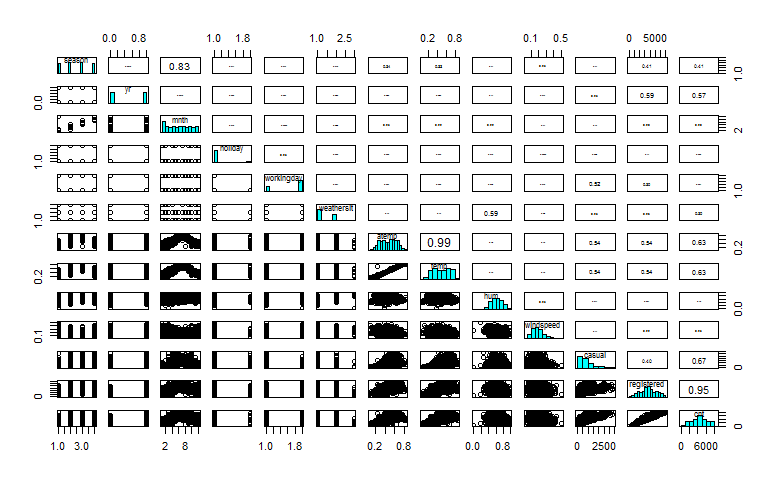
\includegraphics[scale=0.6]{figures/scatterplot.png}
		\caption{Scatterplot matrix of the bike sharing (daily) dataset}
		\label{fig:scatterplot}
	\end{figure}
	
	As we can see from Figure \ref{fig:scatterplot}, there are 0.99 correlation between temp and atemp, 0.95 correlation between registered and cnt, and 0.83 correlation between season and mnth.
	
	High correlation between two variables means that as one variable rises or falls, the other variable rises or falls as well. Since we don't want attributes with high correlation in our dataset, we can pick one attribute from each pair with high correlation.
	
	On the other side, attributes with high correlations to cnt can be good predictors for the bike rental counts. From the last column of Figure \ref{fig:scatterplot}, we obtained a list of attributes with high correlations to cnt in decreasing order: 
	\begin{table}[H]
		\centering
		\begin{tabular}{| l | l | l | l | l | l|}
			\hline
			& registered & casual & temp/atemp & yr & season\\
			\hline
			 correlation to cnt& 0.95 & 0.67 & 0.63 & 0.57 & 0.41\\
			\hline
			%	registered~ &
		\end{tabular}
		\caption{Correlations to cnt in decreasing order}
	\end{table}
	
    To further explore the correlations between variables, we plotted a heat map with hierarchical clustering. 
	\begin{figure}[H]
		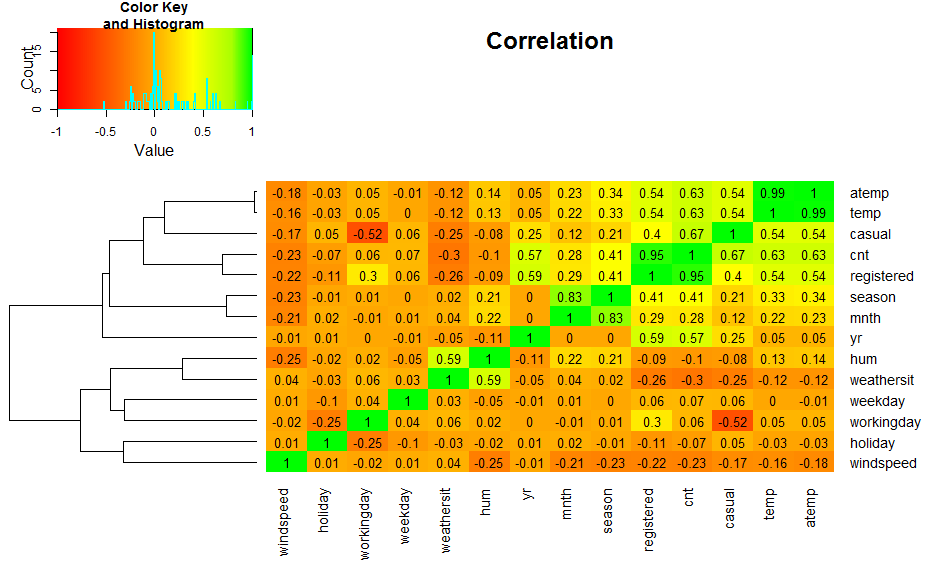
\includegraphics[scale=0.6]{figures/correlation.png}
		\caption{Heat map of the bike sharing (daily) dataset}
		\label{fig:correlation}
	\end{figure}
	From Figure \ref{fig:correlation}, we found that workingday has a negative correlation with casual users (-0.52) which corresponds to the intuition that more casual users go out biking when it is not workingday. 
	
	Moreover, the hierarchical clustering grouped atemp and temp, cnt and registered, season and month, hum and weathersit, weekday and workingday together in the lowest level.  If we want two clusters from the hierarchical clustering, we will get atemp, temp, casual, cnt, registered, season, mnth, yr as one cluster; and hum, weathersit, weekday, workingday, holiday, windspeed as the other cluster.
	
	These correlations give us an insight about the dataset. 	Based on the above observations, we decided to further investigate on the following relationships: 1) temp/weathersit to cnt, 2) hr/workingday (weekday and non-holiday) to cnt,  3)season/mnth to cnt, 4) registered to casual. 
	
	
	\paragraph*{Explore 1. temp/weathersit to cnt} Most likely, temperature and weather influence the bike demand. We thus plotted temp against daily cnt with weather information:
	\begin{figure}[H]
		\centering
		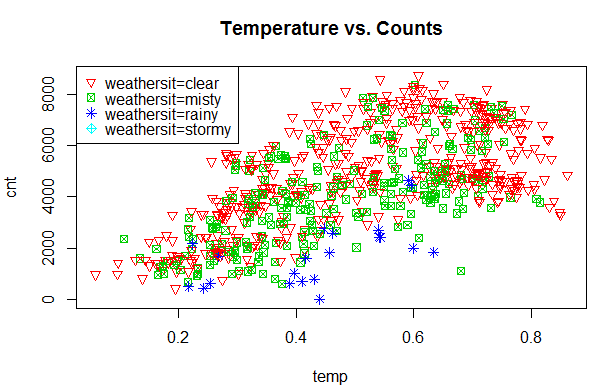
\includegraphics[scale=.85]{figures/temp_counts.png}
	\end{figure}
	
	The rental bike counts increases when the temperature increases. With the same temperature, the better the weather is, the more bike rental counts are.
	
	To compare the effects of feeling temperature and temperature on bike rental demand, we plotted atemp against the average cnt and temp against the average cnt:
	
	\begin{figure}[H]
		\centering
		\begin{minipage}{.44\textwidth}
			\centering
			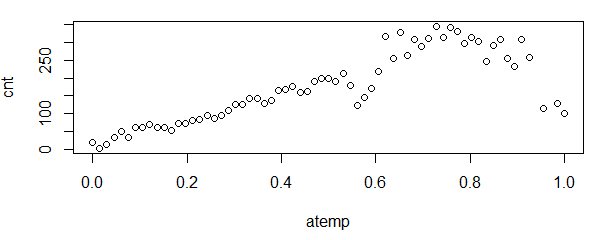
\includegraphics[width=\linewidth]{figures/atemp_cnt.png}
			\caption{Atemp against average cnt}
			\label{fig:atemp}
		\end{minipage}%
		\begin{minipage}{.44\textwidth}
			\centering
			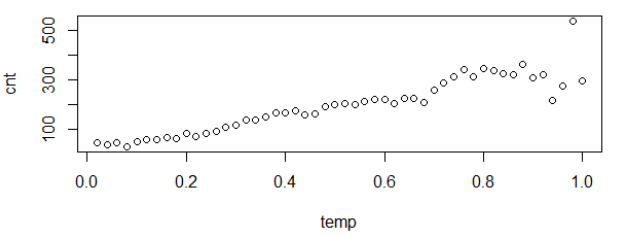
\includegraphics[width=\linewidth]{figures/temp_cnt.png}
			\caption{Temp against average cnt}
			\label{fig:temp}
		\end{minipage}
	\end{figure}
   We can confirm the high linear correlation between temp and cnt from Figure \ref{fig:temp} since the plot is most linear. On the other hand, we can see from Figure \ref{fig:atemp} that the bike rental demand is the highest at atemp$=0.7$, it start to decrease when atemp exceeds 0.7. 
	
	\paragraph*{Explore 2. hr/workingday (weekday and non-holiday) to cnt} The hourly bike rental demand probably shows a different pattern on weekdays and weekends. Many people rent bikes to work on weekdays, and other people rent bikes for leisure on weekends. To investigate if this affects the bike rental demand, we first plotted the counts on a typical week:
	\begin{figure}[H]
		\centering
		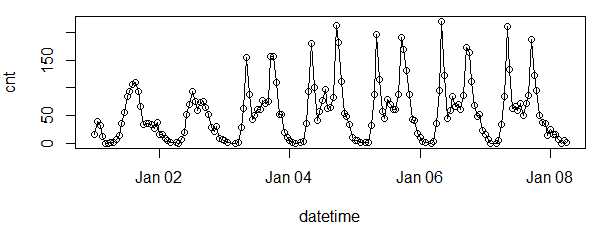
\includegraphics[scale=.9]{figures/week_cnt.png}
		\caption{A typical week of bike rental counts (Sat.- Fri.)}
		\label{fig:typical_week}
	\end{figure}
 We can see that the bike demand is different on weekdays and weekends in Figure \ref{fig:typical_week}. To check if it is true generally, we plotted the average hourly counts conditioned on day of the week from the whole dataset.
	\begin{figure}[H]
		\centering
		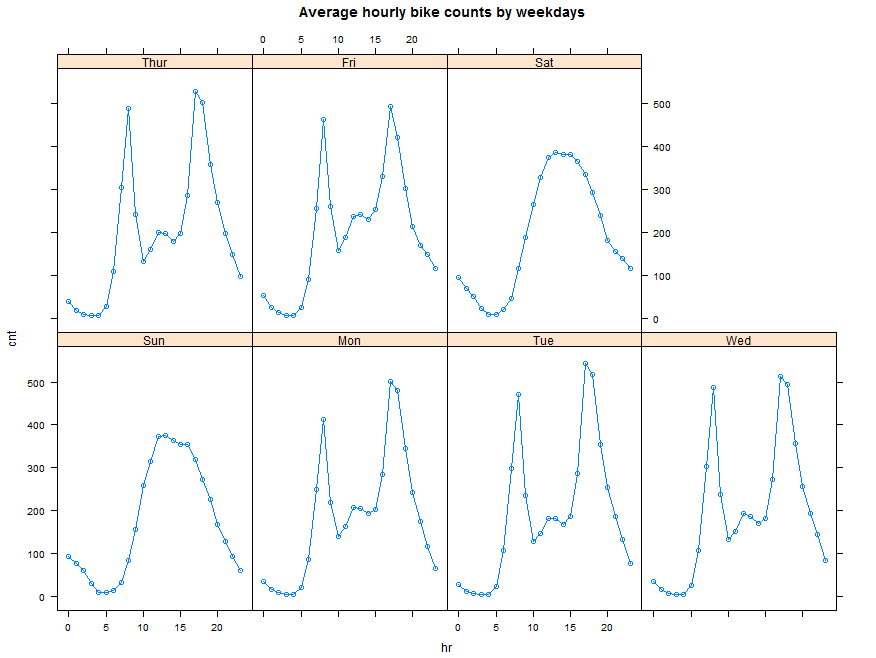
\includegraphics[scale=.5]{figures/hr_weekday.png}
	\end{figure}
	In general, there are two peaks of bike rental during weekdays: around 8-9am and around 5-6pm when people go to work and get off work. On the other hand, the peak bike rentals happen from 12pm to 4pm on weekends when people go outdoors for leisure. 
	
	A natural question to ask here is that what's the bike rental demand is on holidays, especially holidays on weekdays?  Is it going to be similar as the pattern of a weekday or that of weekends? To answer this question, we plotted the average hourly counts conditioned on day of the week AND if it's a holiday.
		\begin{figure}[H]
			\centering
			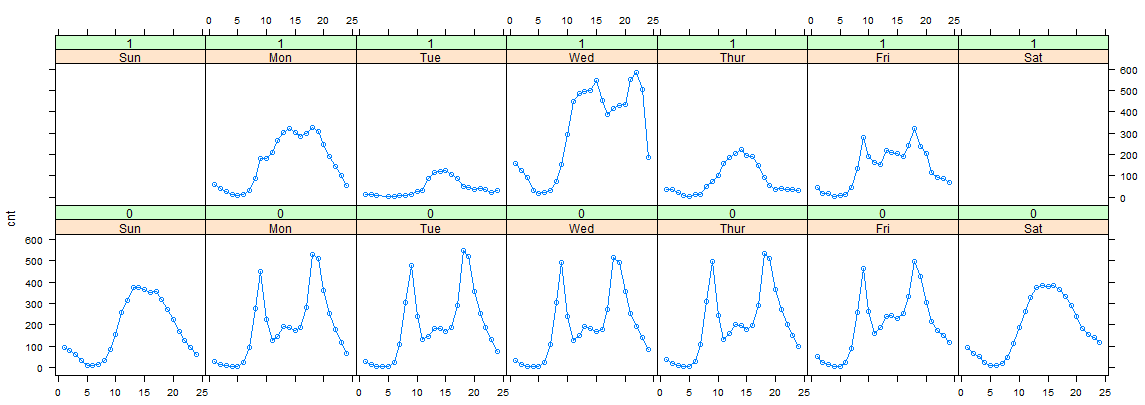
\includegraphics[scale=.5]{figures/hr_weekday_holiday.png}
			\caption{Average hourly bike rental on different weekdays and holidays (1 indicates holiday, 0 indicates non-holiday)} 
			\label{fig:weekday_holiday}
		\end{figure}
		
	Here are the observations from Figure \ref{fig:weekday_holiday}:
	\begin{enumerate}
		\item There is no holiday on weekends from the dataset since the plot of bike rental on Sunday and Saturday with holiday=1 are empty.
		\item Whenever there is a holiday on weekdays, the bike rental shows very different pattern than that of usual weekdays. It can be similar to the weekends' bike rental pattern with lower counts (Monday, Tuesday and Thursday in Figure \ref{fig:weekday_holiday}) or a combination of weekdays' pattern and weekends' pattern (Monday and Friday in Figure \ref{fig:weekday_holiday}). 
	\end{enumerate}
	
 Therefore, workingday (weekday and non-holiday) is a good predictor for the hourly bike counts as the following graph shows: 
	\begin{figure}[H]
		\centering
		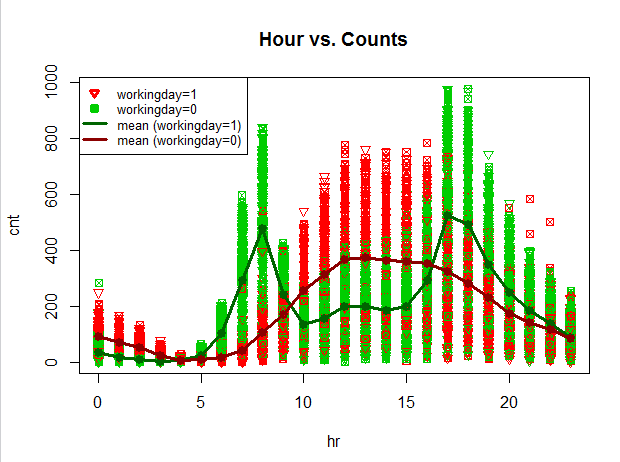
\includegraphics[width=\linewidth]{figures/hr_cnt.png}
	\end{figure}
	
	The bike rentals are concentrating from 7am to 9pm on all days.  The peak rental occurs at 8-9am and 5-6pm on workingdays and occurs from 10am to 4pm on non-workingdays. 
	
	%From this, a bold guess is that more registered people rent on workingdays, and more casual users rent on non-working days. We confirmed this by the following conditional plot.
	
	
	\paragraph*{Explore 3. mnth/season to cnt} Let’s see if bike rental demand depending on the month\ season. To see the relationship of month and bike rental counts, we plotted a boxplot: 
	\begin{figure}[H]
		\centering
		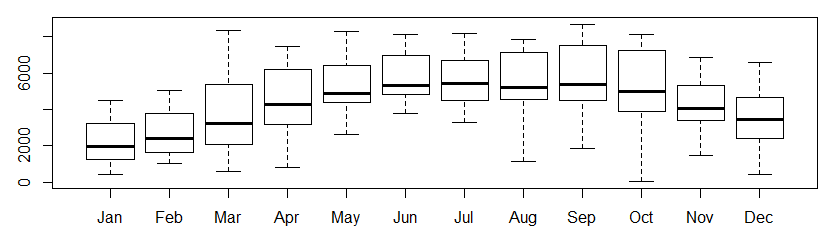
\includegraphics[width=\linewidth]{figures/month_count.png}
		\caption{Boxplot of counts on different months}
	\end{figure}
	The bike rental demand is the lowest in January and is the highest from May to October. To see if the bike rental patterns are similar among months, we plotted a coplot of hourly bike counts conditioned on month.
	
	\begin{figure}[H]
		\centering
		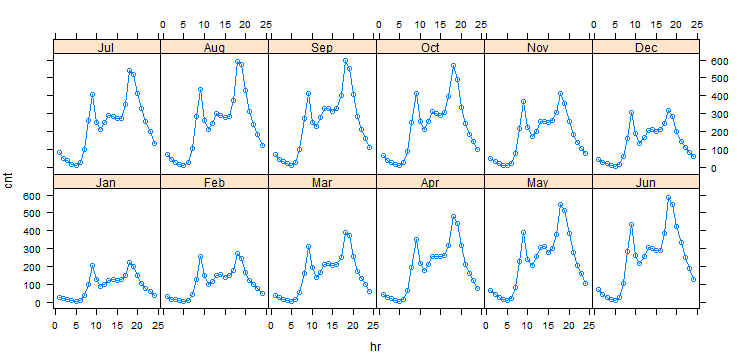
\includegraphics[width=\linewidth]{figures/cnt_hr_mnth.png}
		\caption{Average hourly bike rental on different month}
	\end{figure}
	The bike rentals are the highest in the month from May to October, and the patterns of hourly rental are similar in these months with  the afternoon peak higher than the morning peak. The difference between the afternoon peak and the morning peak might due to the casual users going out biking in the afternoon during the summer.  From November to February, the bike rentals are low and the morning peak has similar counts as that of the afternoon peak. 
	
	Next, we investigated the relationship of season with bike rental counts. We first plotted a coplot of hourly counts conditioned on season:
	
		\begin{figure}[H]
			\centering
			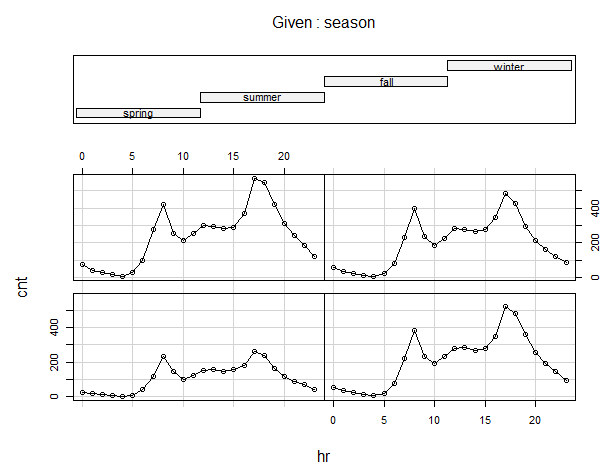
\includegraphics[width=\linewidth]{figures/coplot_season.png}
			\caption{Coplot of hourly counts conditional on season}
		\end{figure}
	
	 The bike demand is the highest in the fall (July to September) and is the lowest in the spring(January to March). The bike rental patterns are similar in the summer, the fall, and the winter with afternoon peak higher than morning peak. 
	 
	 We then used parallel coordinate plots in Ggobi to compare all attributes in different seasons:
	 
	 \begin{figure}[H]
	 	\centering
	 	\begin{minipage}{.5\textwidth}
	 		\centering
	 		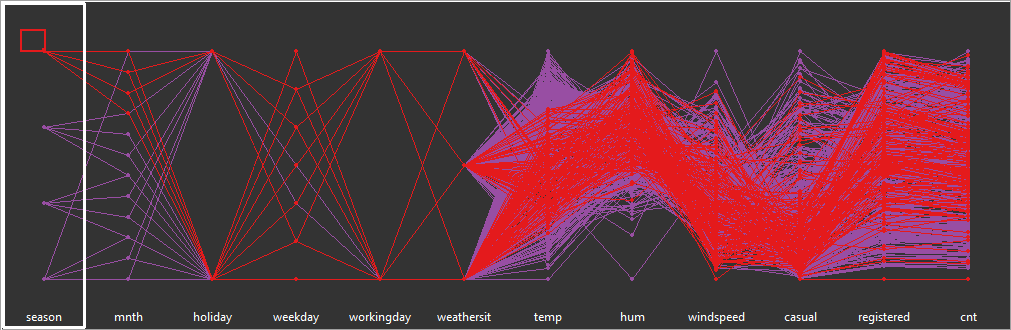
\includegraphics[width=\linewidth]{figures/spring_pcor.png}
	 		\caption{Spring}
	 	\end{minipage}%
	 	\begin{minipage}{.5\textwidth}
	 		\centering
	 		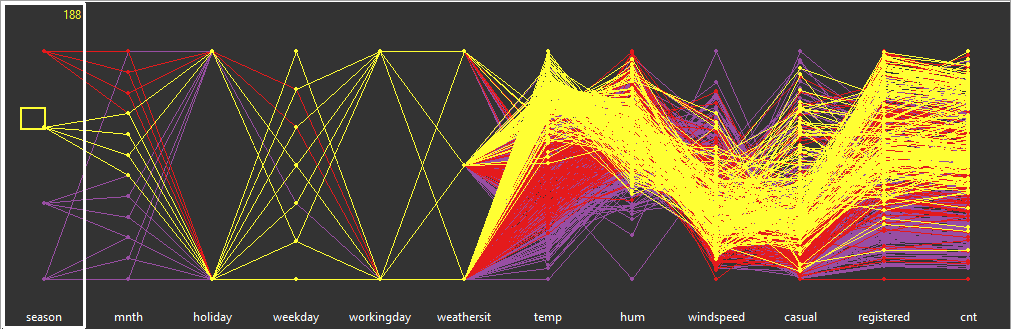
\includegraphics[width=\linewidth]{figures/summer_pcor.png}
	 		\caption{Summer}
	 	\end{minipage}
	 \end{figure}
	 
	 \begin{figure}[H]
	 	\centering
	 	\begin{minipage}{.5\textwidth}
	 		\centering
	 		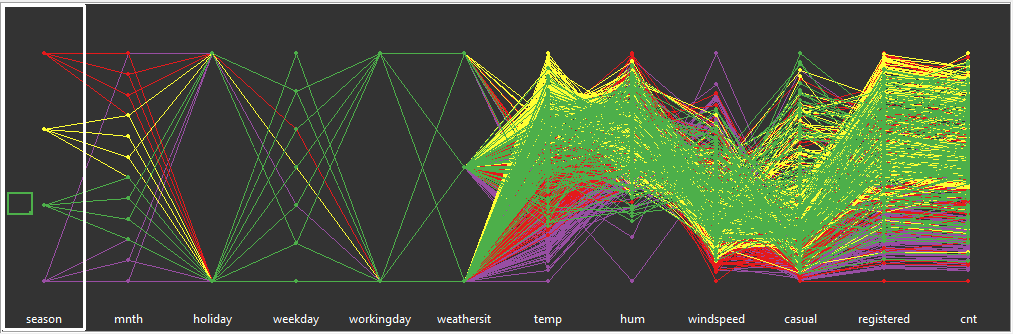
\includegraphics[width=\linewidth]{figures/fall_pcor.png}
	 		\caption{Fall}
	 	\end{minipage}%
	 	\begin{minipage}{.5\textwidth}
	 		\centering
	 		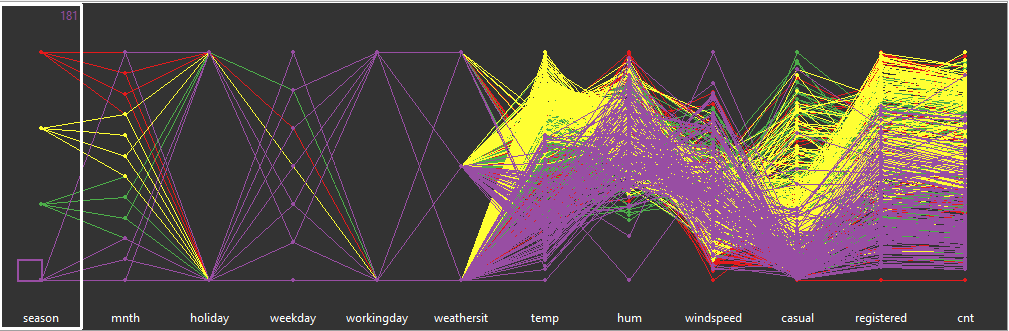
\includegraphics[width=\linewidth]{figures/winter_pcor.png}
	 		\caption{Winter}
	 	\end{minipage}
	 \end{figure}
	From the above plots, we noticed that casual users' bike rental demand are different than that of registered users in different seasons. The demand pattern is summarize in the following table:
	
	\begin{table}[H]
		\centering
		\begin{tabular}{|l|l|l|l|l|}
			\hline
			Season & 	Spring & Summer & Fall & Winter\\ \hline
			Registered & median, high & median, high & median, high & low, median\\
			Casual & low & low, median, high & low, median & low \\ \hline
		\end{tabular}
		\caption{Bike rental demand of casual/registered users in different season}
	\end{table}
    %It seems that month will give more accurate information than season in the prediction. Since these two attributes are highly correlated, we will keep month in our experiment.	
		
	\paragraph*{Explore 4. workingday to registered/casual}
	We found in Explore 3 that casual users behave differently than registered users in different seasons. To see if workingdays contribute to the difference, we plotted a coplot of hourly counts conditioned on season with colored workingdays.
	 \begin{figure}[H]
	 	\centering
	 	\begin{minipage}{.5\textwidth}
	 		\centering
	 		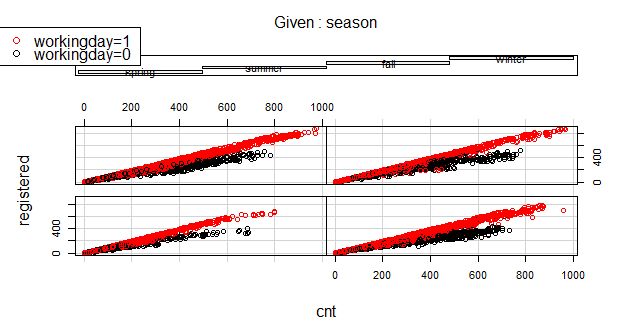
\includegraphics[width=\linewidth]{figures/registered_cnt_season.png}
	 		\caption{Registered-cnt$|$season}
	 		\label{fig:registered-cnt}
	 	\end{minipage}%
	 	\begin{minipage}{.5\textwidth}
	 		\centering
	 		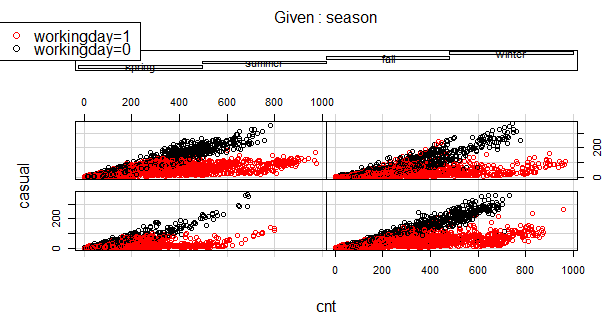
\includegraphics[width=\linewidth]{figures/casual_cnt_season.png}
	 		\caption{Casual-cnt$|$season}
	 		\label{fig:casual-cnt}
	 	\end{minipage}
	 \end{figure}
	 From Figure \ref{fig:registered-cnt} and Figure \ref{fig:casual-cnt}, we can see that registered users and casual users behave differently on workingdays and non-workingdays. More registered users rent bike on workingdays, and more casual users rent bike on non-working days.
	 A coplot on registered against casual conditioned on the month can explain this difference even better:
	 	\begin{figure}[H]
	 		\centering
	 		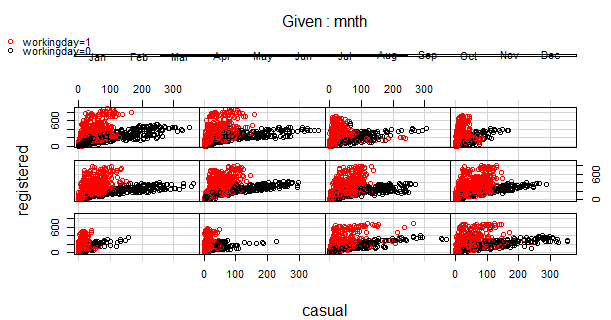
\includegraphics[scale=.9]{figures/coplot_registered_casual_mnth.png}
	 		\caption{Coplot of registered-casual$|$ mnth colored on workingday}
	 		\label{fig:registered_casual}
	 	\end{figure}
	In Figure \ref{fig:registered_casual}, registered and casual almost have a linear correlation on the non-workingday (black dots). But there is no strong linear correlation between the two on workingdays(red dots). This suggests us that building separated models for registered and casual on workingday and non-workingday can improve the prediction of the total counts .
	
	To further explore the difference between casual and registered users, we plotted hourly bike rental counts for casual users and for registered users in a daily basis for the whole dataset. Here are some interesting findings:
	\begin{enumerate}
		\item In winter, less casual users go out biking on weekdays. But the amount of casual users renting bikes on weekends doesn't reduce much from the summer to the winter. 
	
		 \begin{figure}[H]
		 	\centering
		 	\begin{minipage}{.5\textwidth}
		 		\centering
		 		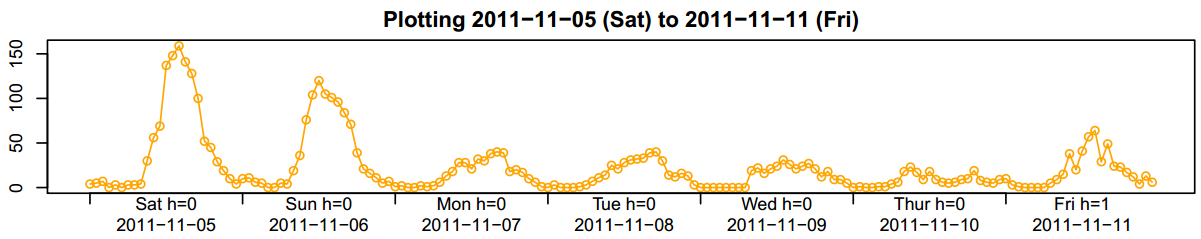
\includegraphics[width=\linewidth]{figures/casual_typical_winter.png}
		 		\caption{Winter - casual users}
		 	\end{minipage}%
		 	\begin{minipage}{.5\textwidth}
		 		\centering
		 		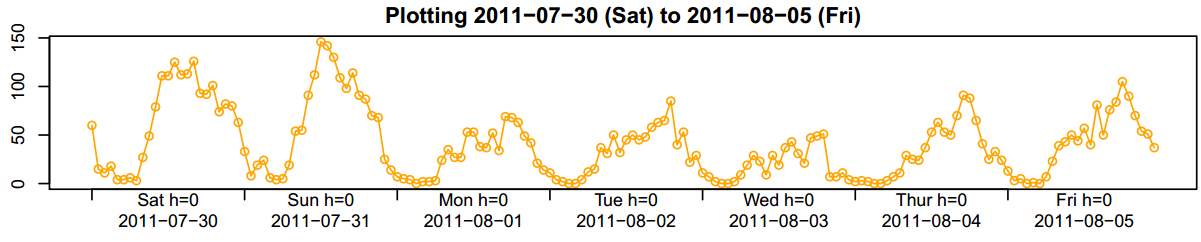
\includegraphics[width=\linewidth]{figures/casual_typical_summer.png}
		 		\caption{Summer - casual users}
		 		%\label{fig:casual-cnt}
		 	\end{minipage}
		 \end{figure}
	 \item Compare to the usual summer weeks, casual users' bike rentals are very low in the week when school starts. This indicates that a large percentage of casual users are students.
	 
	 	 \begin{figure}[H]
	 	 	\centering
	 	 	\begin{minipage}{.5\textwidth}
	 	 		\centering
	 	 		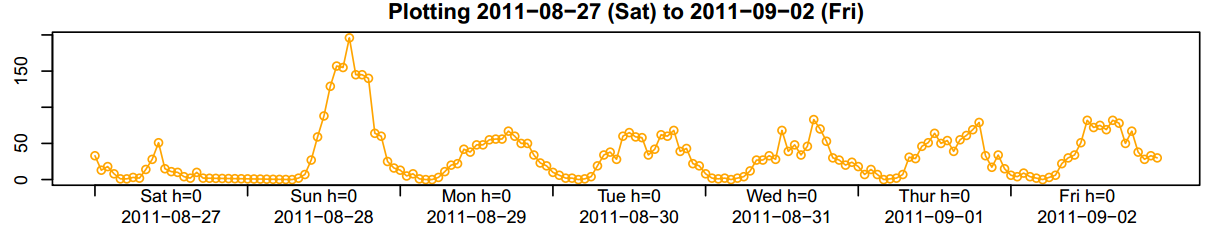
\includegraphics[width=\linewidth]{figures/casual_week_before_school.png}
	 	 		\caption{The week before school starts - casual users}
	 	 	\end{minipage}%
	 	 	\begin{minipage}{.5\textwidth}
	 	 		\centering
	 	 		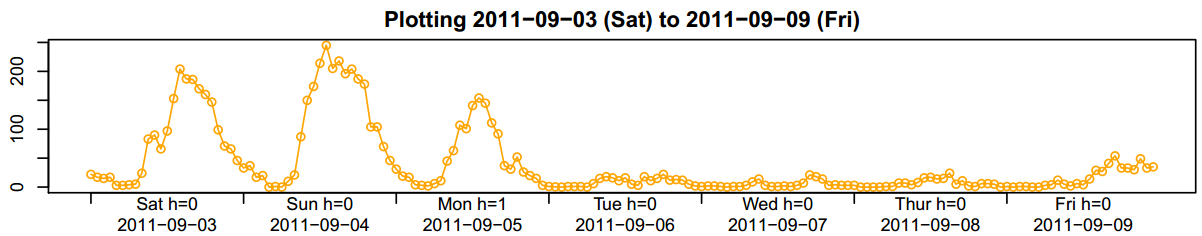
\includegraphics[width=\linewidth]{figures/casual_school_start.png}
	 	 		\caption{The week when school starts - casual users}
	 	 		%\label{fig:casual-cnt}
	 	 	\end{minipage}
	 	 \end{figure}

	\item Christmas is an atypical week for casual users' bike rentals. 
		 \begin{figure}[H]
		 	\centering
		 	\begin{minipage}{.5\textwidth}
		 		\centering
		 		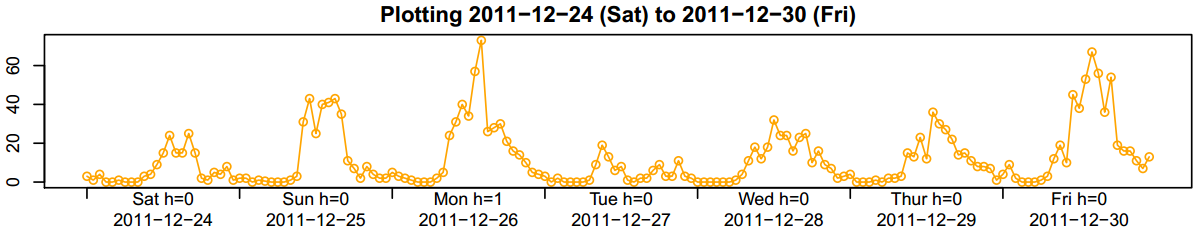
\includegraphics[width=\linewidth]{figures/casual_chritmas_2011.png}
		 		\caption{Christmas 2011- casual users}
		 	\end{minipage}%
		 	\begin{minipage}{.5\textwidth}
		 		\centering
		 		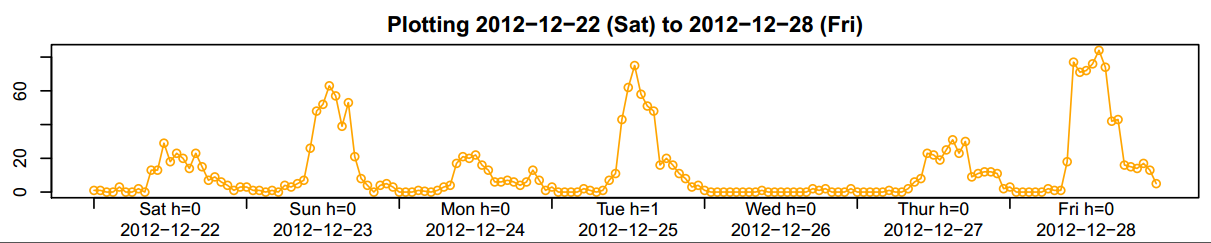
\includegraphics[width=\linewidth]{figures/casual_christmas.png}
		 		\caption{Christmas 2012- casual users}
		 		%\label{fig:casual-cnt}
		 	\end{minipage}
		 \end{figure}
		 
		 \item The bike rentals for registered users don't change that much from the summer to the winter on weekdays. However, more registered users go bike on weekends during the summer.
		 	\begin{figure}[H]
		 		\centering
		 		\begin{minipage}{.5\textwidth}
		 			\centering
		 			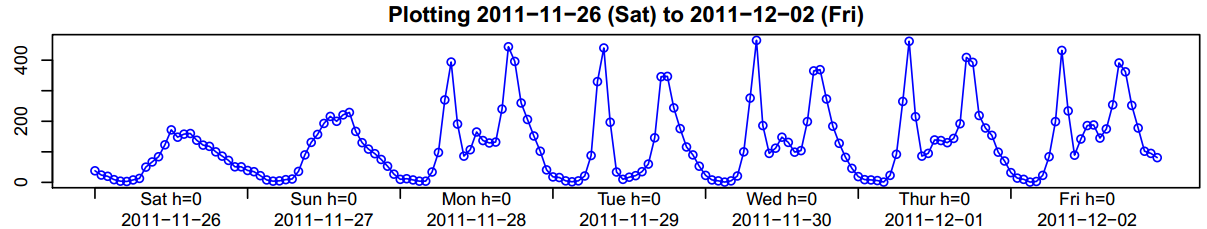
\includegraphics[width=\linewidth]{figures/registered_typical_winter.png}
		 			\caption{registered typical winter}
		 		\end{minipage}%
		 		\begin{minipage}{.5\textwidth}
		 			\centering
		 			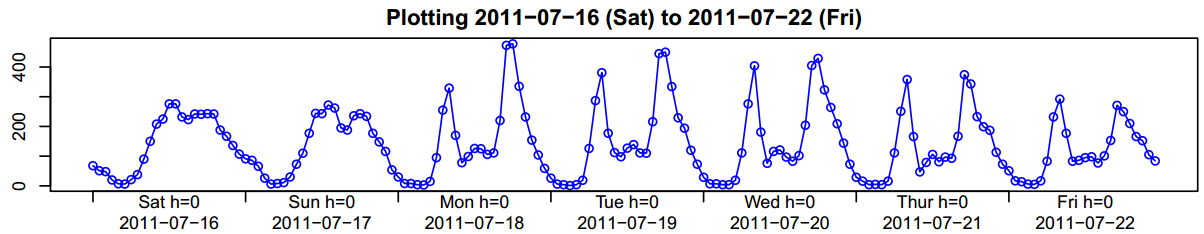
\includegraphics[width=\linewidth]{figures/registered_typical_summer.png}
		 			\caption{registered typical summer}
		 			%\label{fig:casual-cnt}
		 		\end{minipage}
		 	\end{figure}
		 	
		\item Christmas is an atypical week for registered users' bike rentals. 
			 \begin{figure}[H]
			 	\centering
			 	\begin{minipage}{.5\textwidth}
			 		\centering
			 		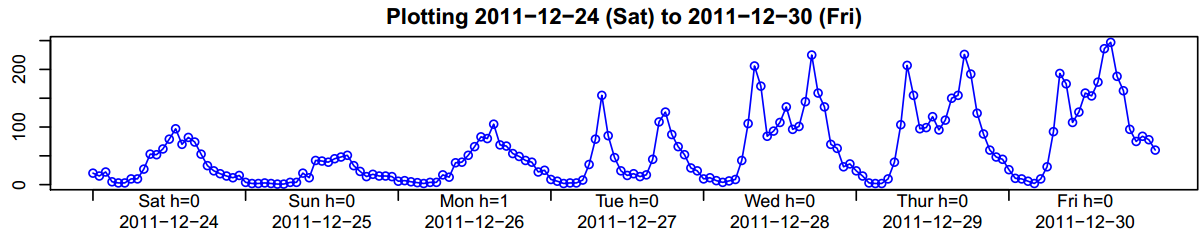
\includegraphics[width=\linewidth]{figures/registered_christmas_2011.png}
			 		\caption{registered chritmas 2011}
			 	\end{minipage}%
			 	\begin{minipage}{.5\textwidth}
			 		\centering
			 		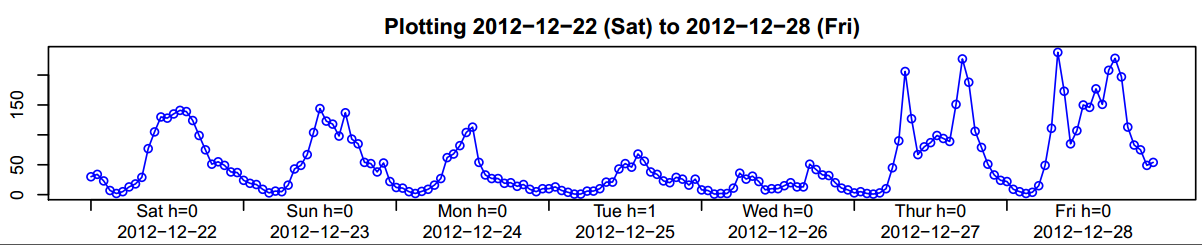
\includegraphics[width=\linewidth]{figures/registered_christmas_2012.png}
			 		\caption{registered christmas 2012}
			 		%\label{fig:casual-cnt}
			 	\end{minipage}
			 \end{figure}
		\end{enumerate}
		
	\paragraph*{Preliminary Conclusion.}	
	In short we have identified strong correlation between counts and these predictors: 1. Temperature 2. Hour of the Day 3. Working Day 4. Month of the Year. 
	
	\subsection{Association Rule Mining}	
	To investigate more about the dataset, we did an association rule mining. The bike sharing dataset contains a mixture of categorical and numeric attributes and therefore need some preparation before using apriori algorithm on it. Here are the steps for our experiment in association rule mining:
    \begin{enumerate}
    	\item We fist removed the unrelated features: instant, dteday.
    	\item We then mapped the seven remaining continuous attributes (temp, atemp, hum, windspeed, registered, casual, and cnt) to ordinal attributes by building suitable categories.
    	\item Next, we coerced the data set to transactions (a binary incidence matrix).
    	\item Finally, we ran Apriori algorithm with support = 0.01, confidence = 0.3.
    \end{enumerate}
	
	After the rule mining, we sorted the rules by lift with "cnt=high" in the right hand side. Here are the top 5 rules: \color{blue}
	\begin{verbatim}
	   lhs                   rhs           support confidence     lift
	   1  {weekday=Sat,                                                  
	   casual=high}      => {cnt=high} 0.03283174          1 3.768041
	   2  {casual=high,                                                  
	   registered=high}  => {cnt=high} 0.02872777          1 3.768041
	   3  {hum=medium,                                                   
	   casual=high}      => {cnt=high} 0.03283174          1 3.768041
	   4  {mnth=Sep,                                                     
	   registered=high}  => {cnt=high} 0.03419973          1 3.768041
	   5  {mnth=Jun,                                                     
	   registered=high}  => {cnt=high} 0.03009576          1 3.768041
	\end{verbatim} \color{black}
    The first rule tells us that when it is Saturday and bike rentals from casual users are high, there will be a large chance that total bike rentals are high.
    
    We also sorted the rules by lift with "registered=high" on the right hand side. The following are the top 5 rules: \color{blue}
	\begin{verbatim}
	   lhs                rhs                  support confidence     lift
	   1  {weekday=Fri,                                                      
	   cnt=high}      => {registered=high} 0.03967168          1 3.673367
	   2  {weekday=Wed,                                                      
	   cnt=high}      => {registered=high} 0.03693570          1 3.673367
	   3  {weekday=Thur,                                                     
	   casual=medium} => {registered=high} 0.01231190          1 3.673367
	   4  {weekday=Thur,                                                     
	   cnt=high}      => {registered=high} 0.04377565          1 3.673367
	   5  {casual=low,                                                       
	   cnt=high}      => {registered=high} 0.12859097          1 3.673367
	\end{verbatim}\color{black}
	in general, these five rules tell us that when it is weekdays, registered is high.
	
	 Finally, we obtained the following top 5 rules by sorting with lift and with "casual=high" on the right hand side: \color{blue}
	\begin{verbatim}
	   lhs                   rhs              support confidence     lift
	   1  {season=summer,                                                   
	   weekday=Sat,                                                     
	   cnt=high}         => {casual=high} 0.01504788          1 16.61364
	   2  {season=summer,                                                   
	   weekday=Sat,                                                     
	   workingday=0,                                                    
	   cnt=high}         => {casual=high} 0.01504788          1 16.61364
	   3  {season=summer,                                                   
	   weekday=Sat,                                                     
	   atemp=medium,                                                    
	   cnt=high}         => {casual=high} 0.01094391          1 16.61364
	   4  {season=summer,                                                   
	   yr=2012,                                                         
	   weekday=Sat,                                                     
	   cnt=high}         => {casual=high} 0.01504788          1 16.61364
	   5  {season=summer,                                                   
	   weekday=Sat,                                                     
	   weathersit=clear,                                                
	   cnt=high}         => {casual=high} 0.01231190          1 16.61364
	\end{verbatim}\color{black}
	Here, we can see that when it is summer weekends and cnt is high, there will be a very large chance that casual users' bike rentals are high.  
	
	Rule 4 attracted our attention since it indicates that ``yr=2012'' can help to predict high bike rental demand from casual users. We therefore plotted hourly casual, registered, and cnt conditioned on yr to compare the difference. 
	
	\begin{figure}[H]
		\centering
		\begin{minipage}{.48\textwidth}
			\centering
			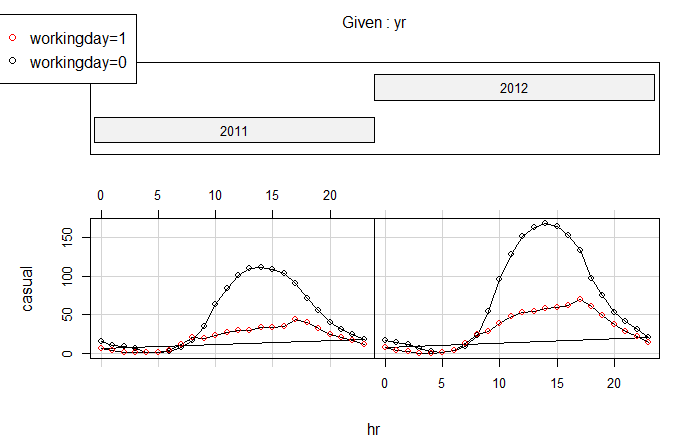
\includegraphics[width=\linewidth]{figures/casual_yr.png}
			\caption{Coplot of casual-hr$|$ yr}
			%\label{fig:registered-cnt}
		\end{minipage}%
		\begin{minipage}{.48\textwidth}
			\centering
			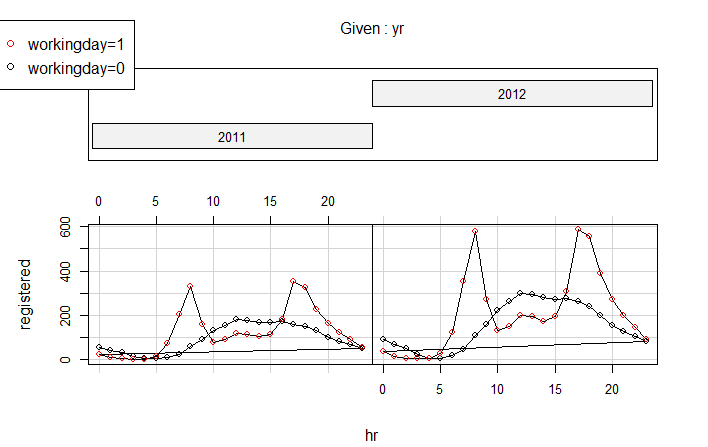
\includegraphics[width=\linewidth]{figures/registered_yr.png}
			\caption{Coplot of registered-hr$|$ yr}
			%\label{fig:casual-cnt}
		\end{minipage}
	\end{figure}
	
		\begin{figure}[H]
			\centering
			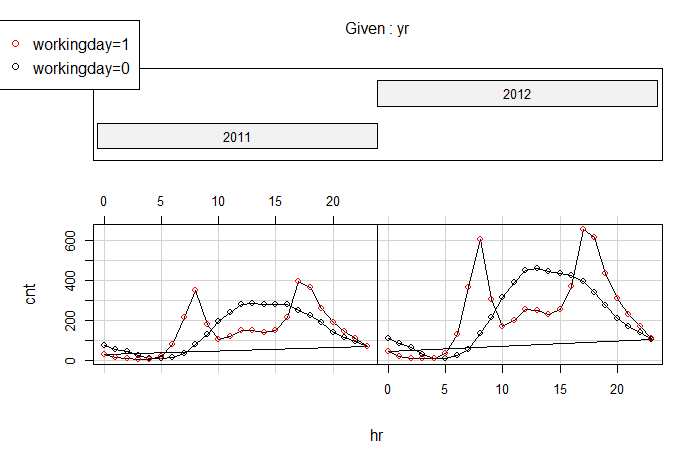
\includegraphics[width=\linewidth]{figures/cnt_year.png}
			\caption{Coplot of cnt-hr$|$ yr}
		\end{figure}
    From the above figures, the bike rental demands from the registered users and the casual users both increase from 2011 to 2012 without changing on the underlying pattern of the rental. Therefore, yr is also a strong predictor for the total counts.
    
    In summary, the association rule mining didn't give us too much more information about the dataset. But it confirmed that casual and registered users behave differently. In addition, it helped us to realize year is also a strong predictor for the bike rental demand. 
	\section{Unsupervised Learning: Data Preprocessing}
	\subsection{Dimension Reduction: PCA }
	\label{sec:dimension-reduction}
	
	\subsection{Data Reduction: Clustering Kmeans + Davies-Bouldi Index}
	\label{data-reduction}
	
	The bike sharing dataset has  17365 data instances for the hourly bike sharing dataset. Instead of dimension reduction to reduce the number of attributes, we can use data reduction to reduce the number of cases. In this section, we consider using clustering methods to group similar cases together. By doing so, we can have a reduced representation for the dataset which produces the same or similar analytical results.
	\subsubsection{Data transformation}
	The k-means clustering uses Euclidean distance to calculate the similarity between instances, therefore the attributes of the input should be continuous numerical values. The bike sharing dataset has a mixture of categorical and numerical values, we thus need some data transformation before running the k-means algorithm.
	
	Instead of using all information to clustering the data, we considered only cluster the daily bike rental patterns. In other words, we fed the hourly counts to the k-means algorithm to group the days with similar counts pattern. To achieve this, we transformed the cnt in hourly dataset into a $713 \times 24$ matrix as follows: \color{blue}
	\begin{verbatim} 
	head(bike.24hourscnt)
 	  hr0 hr1 hr2 hr3 hr4 hr5 hr6 hr7 hr8 hr9 hr10 hr11 hr12 hr13 hr14 hr15
	1  16  40  32  13   1   1   2   3   8  14   36   56   84   94  106  110
	2  17  17   9   6   3  NA   2   1   8  20   53   70   93   75   59   74
	3   5   2  NA  NA   1   3  30  64 154  88   44   51   61   61   77   72
	4   5   2   1  NA   2   4  36  94 179 100   42   57   78   97   63   65
	5   6   6   2  NA   2   3  33  88 195 115   57   46   79   71   62   62
	6  11   4   2  NA   1   4  36  95 219 122   45   59   84   67   70   62
	  hr16 hr17 hr18 hr19 hr20 hr21 hr22 hr23
	1   93   67   35   37   36   34   28   39
	2   76   65   53   30   22   31    9    8
	3   76  157  157  110   52   52   20   12
	4   83  212  182  112   54   48   35   11
	5   89  190  169  132   89   43   42   19
	6   86  172  163  112   69   48   52   23
	\end{verbatim} \color{black}
	Our goal is using k-means and DBI to find a proper way to cluster the dataset. For example, we want to find some clusters as the following graph shows:
	\begin{figure}[H]
		\centering
		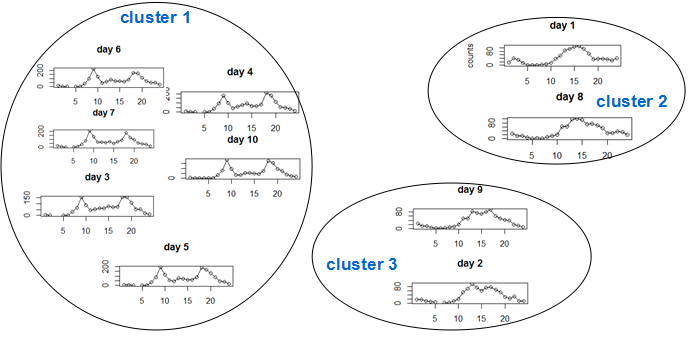
\includegraphics[scale=.8]{figures/cluster_goal.png}
		\caption{One example of our goal for k-means}
	\end{figure}
	
	
	\subsubsection{Fill in missing values}
	As we can see from the last section, the bike sharing dataset has lots of missing values. For example, the bike counts on the second day at hour 5 is missing. A check shows that there are 76 days with missing values, and 14 days with more than 1 missing values. 
	
	We can fill up the missing values by three ways with the ``zoo'' package:
	\begin{enumerate}
		\item fill the missing value by the last observation carried forward (locf)
		
		\item fill the missing value by linear interpolation (linear)
		
		\item fill the missing value by cubic spline (spline)
	\end{enumerate}
	To compare the performances of these three methods, we removed the data of hour (3,5,6,10,11,15,16) on day 1 and day 10. Then we filled the missing values with the three filling methods. Finally, we computed the Root Mean Square Error for the comparison. 
	\begin{figure}[H]
		\centering
		\begin{minipage}{.45\textwidth}
			\centering
			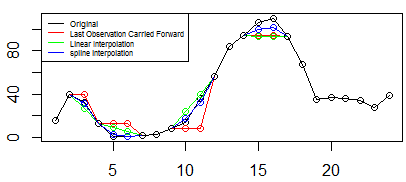
\includegraphics[width=\linewidth]{figures/day1_missing_value.png}
			\caption{3 filling methods on day 1, rmse(locf)=8.093207, rmse(linear)=5.273207, rmse(spline)=2.306192}
			%\label{fig:registered-cnt}
		\end{minipage}%
		\begin{minipage}{.42\textwidth}
			\centering
			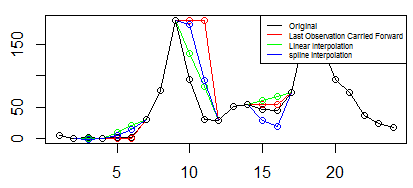
\includegraphics[width=\linewidth]{figures/day10_missing_value.png}
			\caption{ 3 filling methods on day 10, rmse(locf)=37.4316, rmse(linear)=15.07681, rmse(spline)=22.98093}
			
			%\label{fig:casual-cnt}
		\end{minipage}
	\end{figure}
 From the root mean square errors of the three methods on workingday (day 10) and non-workingday (day 1), we found linear or spline interpolation fit our dataset better. We chose a combination of linear and spline interpolation to fill the whole dataset: we first used cubic spline to fill the dataset, then the rest miss values are filled by linear interpolation.
\subsubsection{K-means}	

After filling up the missing values, we performed k-means from 2 to 9 clusters. The following is the plot of these clusters with the first two principle components as the axis.
	\begin{figure}[H]
		\centering
		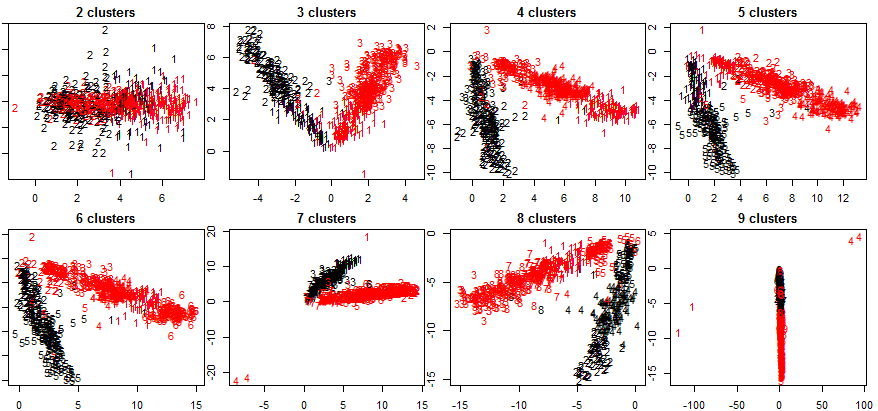
\includegraphics[scale=.65]{figures/kmeans_workingday.png}
		\caption{Clusters with workingday (red) and non-workingday (black)}
	\end{figure}

We can see that workingday give a good separation of clusters when there are 3 to 8 clusters. To investigate what are other attributes used to separate the data in k-means, we printed out the average temperature on each cluster with the workingday. We use k=4 as an example: \color{blue}
\begin{multicols}{2}
	\begin{verbatim}
Cluster #1
Working days: 246 (100%)
Total days: 246
Cluster #2
Working days: 107 (53.8%)
Total days: 199
Cluster #3
Working days: 4 (2.84%)
Total days: 141
Cluster #4
Working days: 143 (98.6%)
Total days: 145
	\end{verbatim}
	\columnbreak
	\begin{verbatim}
Cluster #1
Avg temperature: 0.4974
Total days: 246
Cluster #2
Avg temperature: 0.3197
Total days: 199
Cluster #3
Avg temperature: 0.5463
Total days: 141
Cluster #4
Avg temperature: 0.5776
Total days: 145
	\end{verbatim}
\end{multicols} 
\color{black}
As we can see, cluster 1 and 4 are mainly composed of workingdays: 100\% in cluster 1, 98.6\% in cluster 4; cluster 3 are mainly composed of non-workingdays (97.26\%).  Cluster 2 is a mixture of workingdays and non-workingdays, but the average temperature in cluster 2 is obviously lower than that in other clusters. Therefore, workingday and temp are good attributes to separate the clusters.

A drawing of average hourly counts on each cluster confirmed our findings:
	\begin{figure}[H]
		\centering
		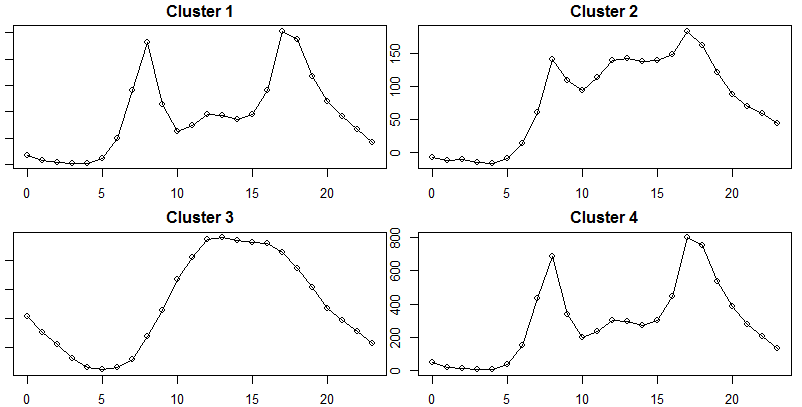
\includegraphics[scale=.65]{figures/kmeans_clusters.png}
		\caption{Average counts plot on each cluster}
	\end{figure}
The following are our observations:

\begin{enumerate}
	\item Cluster 1 and cluster 4 are having the pattern of workingdays. However, the counts in cluster 1 is lower which indicates cluster 1 is representative for days with the lower temperature.
	\item Counts in cluster 2 look like a mixture of working and non-working days with low counts. It is more likely in the winter.
	\item Cluster 3 are high counts with the pattern of non-workingday.
\end{enumerate}

\subsubsection{DBI}
To determine how many clusters we should choose for the k-means, we used Davies-Bouldin index method. After 8 runs, we found the following graph is representative with the average minimum DBI=8.
	\begin{figure}[H]
		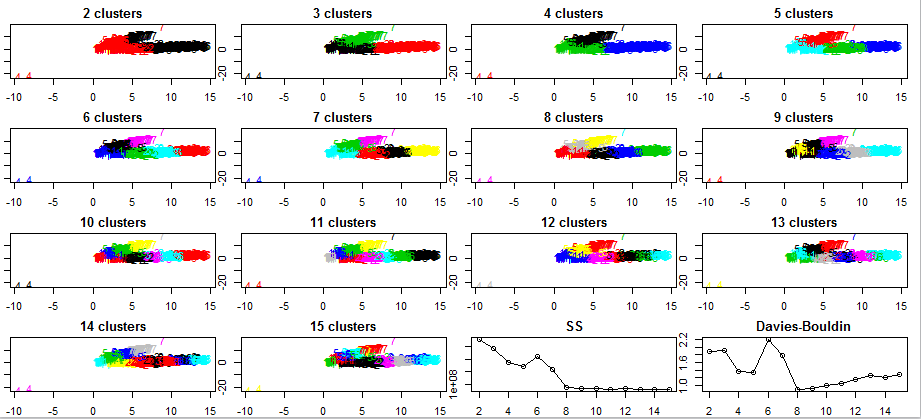
\includegraphics[scale=.65]{figures/dbi_8.png}
		\caption{2 to 15 clusters with DBI}
	\end{figure}
	
	\subsection{Data Reduction: Outlier Detection}
	Another way to reduce the data is to remove extreme values. By doing so, we can find a better representation of the data. In this section, we consider to use Interquartile Range ( ``A filter for detecting outliers and extreme values based on interquartile ranges.'') in WEKA  and lofactor in R to detect outliers.  
	
	We first tried Interquartile Range filter in WEKA. This ``smart'' algorithm gave us 21 outliers which are all holidays:
		\begin{figure}[H]
			\centering
			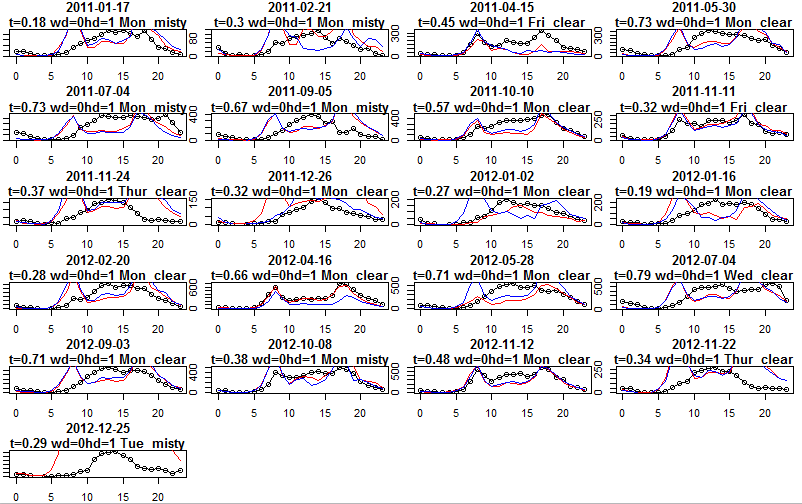
\includegraphics[scale=.65]{figures/outlier_weka_holliday.png}
			\caption{Outliers detected by WEKA (black line is the count on this day, red is 7 days ago, black is 7 days after)}
		\end{figure}
	We can see that the black lines are very different than red lines (7 days ago) and blue lines (7 days after) in all 21 days. This is because all of these 21 holidays are happening on weekdays. When the holiday happens on weekdays, the bike rental pattern is more similar to that of non-workingdays.
	
	We decided to remove the holiday information in the dataset and ran Interquartile Range filter again. Then we obtained the following days as outliers:
		\begin{figure}[H]
			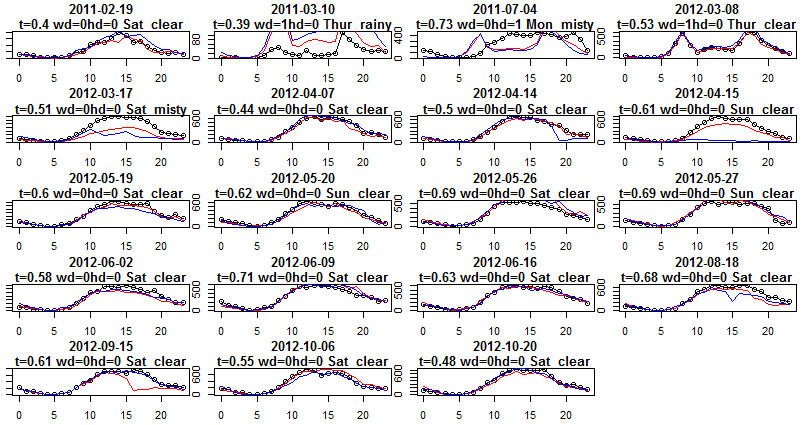
\includegraphics[scale=.65]{figures/outlier_weka_nonholliday.png}
			\caption{outliers detected by WEKA without holiday information}
			\label{fig:outlier_weka}
			%\label{fig:outlier_weka)
		\end{figure}
	It seems that only on 2011-03-10 and 2011-07-04, the black lines are different than red/blue lines from Figure \ref{fig:outlier_weka)}.
	
	We also tried the lofactor outlier detector in R:
	\begin{figure}[H]
		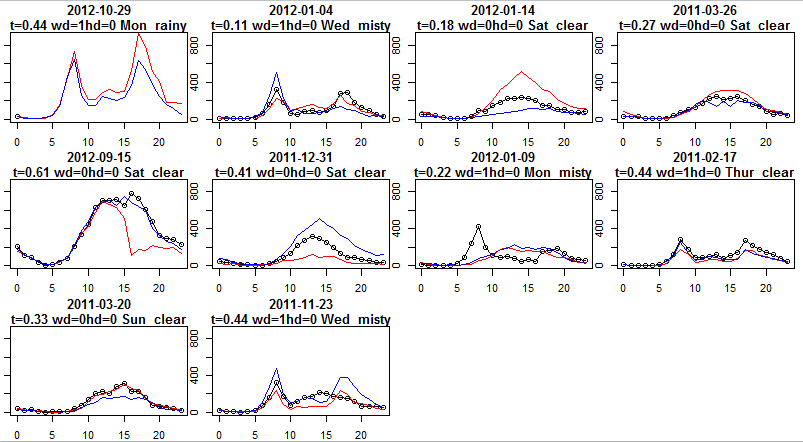
\includegraphics[scale=0.7]{figures/outlier_R.png}
	\end{figure}
 We noticed that on 2012-10-29, there is a big storm based on Gama's paper about event detection \cite{dataset}, the detector in R caught this. We then used the events detected in Gama's paper as a baseline comparison for our outlier detectors. 

 	\begin{figure}[H]
 		\centering
 		\begin{minipage}{.48\textwidth}
 			\centering
 			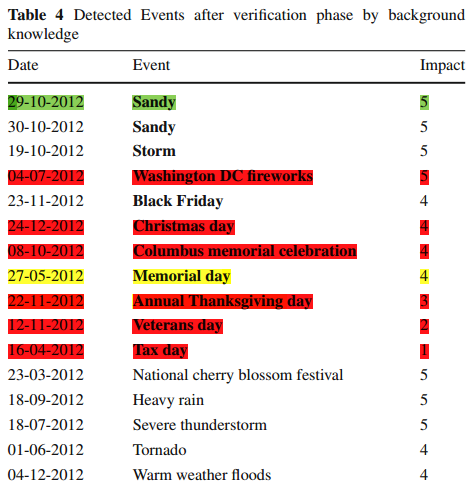
\includegraphics[width=\linewidth]{figures/event_Gama1.png}
 			%\label{fig:registered-cnt}
 		\end{minipage}%
 		\begin{minipage}{.48\textwidth}
 			\centering
 			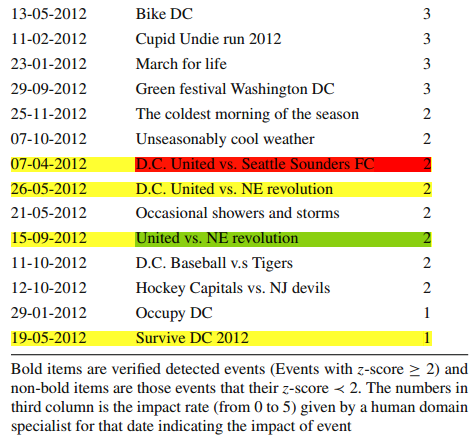
\includegraphics[width=\linewidth]{figures/event_Gama2.png}
 			%\caption{Coplot of registered-hr$|$ yr colored on workingday}
 			%\label{fig:casual-cnt}
 		\end{minipage}
 		5\caption{red: events found by detector in WEKA with holiday information, yellow: events found by detector in WEKA without holiday information, green: events found by detector in R with holiday information}
 	\end{figure}
 	As we can see from the above table, our outlier detectors do help find some events which influence the bike rental. We can eliminate these days found by the three outlier detectors. However, we are also removing points which might be useful since there might be a lot of false alarms on the days detectors found.  
 	
 	A better way to approach is separate data into day of events or not and train models separately on these two datasets. When a new data instance come, we first let the detector decide if it is event day, and pass it to correct model.
	
\section{Experimental Design}
\label{sec:experimental-design}



\section{Data preparation}
WILL MOST LIKELY NEED TO MOVE THIS SOMEWHERE ELSE AND JUST REFER TO IT HERE.

The relationship between \texttt{atemp} and \texttt{cnt} is non-linear, as can be seen from GRAPHREF. However, there seems to be a peak temperature for bike rentals at around PEAKTEMP. Hence, it would make sense to define a new variable corresponding to the (absolute value) difference between the current temperature and this ``ideal temperature''. Let \texttt{atempdiff} be defined as:
\begin{verbatim}
atempdiff <- abs(atemp - PEAKTEMP)
\end{verbatim}
Then, the relationship between \texttt{atemptdiff} and \texttt{cnt} is roughly linear as we can see from OTHERGRAPH.

IDEM with \texttt{hum}, except the ``ideal humidity'' is at around 0.2.

\section{Data Imputation}

We observed that some rows were missing in the hourly Bike Sharing datasets. In total, 165 observations were missing in 76 different days. We decided that it would be wise to impute the missing data, since it could help build a better regression model. Moreover, having no missing data would make the R programming significantly easier since the dataset structure would become more regular and hence much easier to work with.

\subsection{Imputation of Numeric Variables}
We decided to use the \texttt{zoo} package to handle data imputation. The numeric variables (i.e. \texttt{temp}, \texttt{atemp}, \texttt{hum}, \texttt{windspeed}, \texttt{casual}, \texttt{registered}, \texttt{cnt}) were imputed using linear interpolation. This was very straightforward and produced results which we deemed acceptable for most variables such as \texttt{temp}, \texttt{atemp}, \texttt{hum} and \texttt{windspeed}. However, for \texttt{casual}, \texttt{registered} and \texttt{cnt}, the imputated data was clearly wrong in a few isolated cases. In the vast majority of the cases, only 1 or 2 observations were missing in a 24-hour period, in which case the linear interpolation was deemed appropriate. In fact, this was the case for 68 out of the 76 days with missing data. However, there were 8 days with a large number of missing observations (between 6 and 23 missing observations per 24-hour period). We decided to investigate visually the results of our imputation method for those days by constructing Figure~\ref{fig:badrows} below.
\begin{figure}[H]
	\centering
	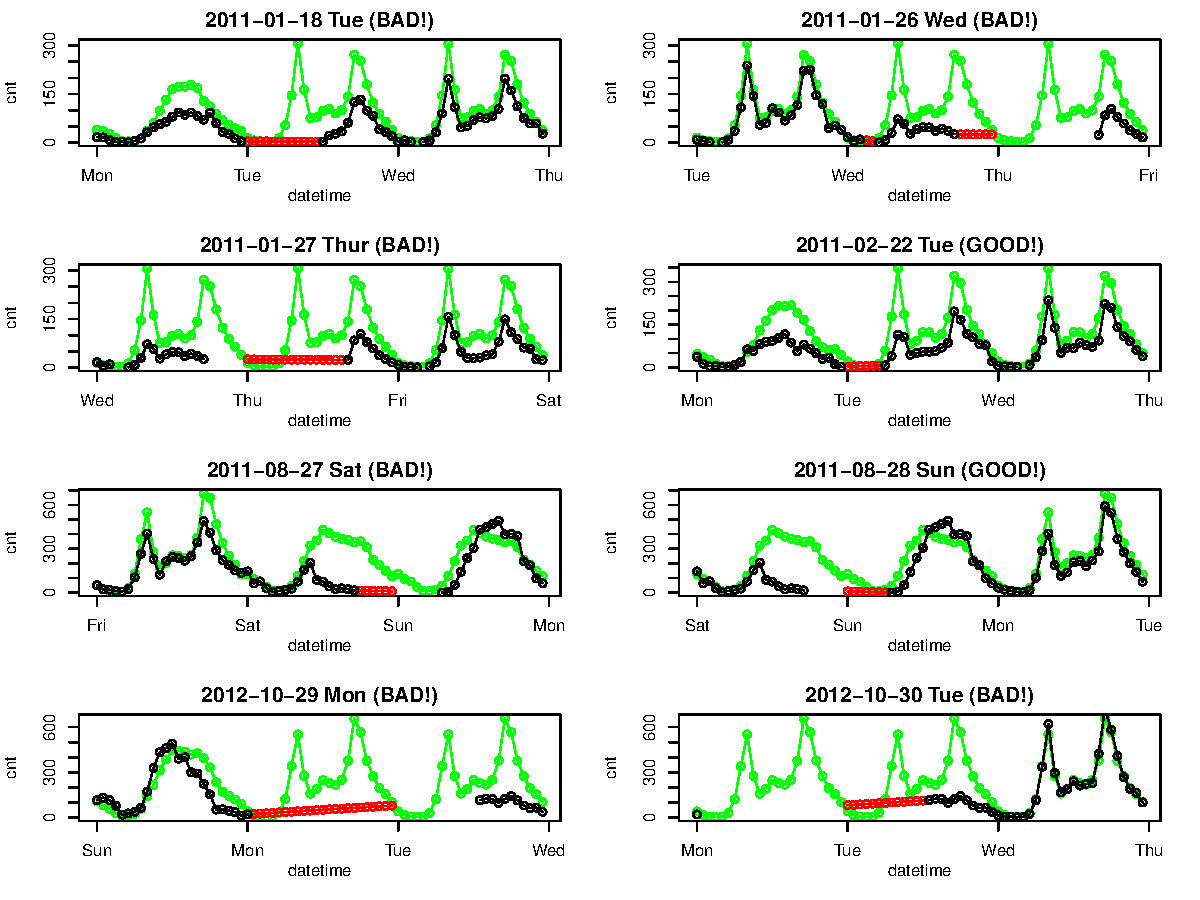
\includegraphics[width=.98\textwidth]{figures/badrows.pdf}
	\caption{Imputation of missing observations of \texttt{cnt} for the 8 days with the highest number of missing data. Each day is plotted along with 24 hours before and 24 hours after, in order to see the continuity between successive days after data imputation. The {\textbf{\color{black}black}} curve represents the actual values of \texttt{cnt} from the dataset. The {\textbf{\color{red}red}} curve are the observations that were imputed using linear interpolation. The {\textbf{\color{green}green}} curve represents the average value of \texttt{cnt} at the same hour on the same day of the week over the same month (the {\textbf{\color{green}green}} curve therefore provides a rough idea of what a typical day looks like and helps us decide if the imputation is acceptable or not).}
	\label{fig:badrows}
\end{figure}
Without much surprise, linear interpolation of \texttt{cnt} produced poor results in 6 out of the 8 cases illustrated in Figure~\ref{fig:badrows}. However, the imputation on dates 2011-02-22 and 2011-08-28 produced good results. Indeed, the missing observations for those two days were during the hours of the night, during which \texttt{cnt} is fairly flat, hence linear interpolation produces acceptable results. On the other hand, the missing observations from the other 6 days appear during the morning, afternoon or evening, during which \texttt{cnt} is highly non-linear. It would still be possible to impute missing data using linear interpolation if very few successive observations (perhaps one or two) were missing, but this is not the case here, which explains the poor results for those 6 days.

At this point, we had a choice to either (1) design more sophisticated imputation methods or to (2) simply discard those 6 days with poor imputation results. Since the vast majority of imputation was successful (70 out of 76 days), we decided that it was best to go with option (2) and simply flag as ``bad rows'' those 6 days from Figure~\ref{fig:badrows} for which imputation of \texttt{cnt} was poor. This allows us later to simply exclude those days completely in the training phase of supervised learning.

\subsection{Imputation of Categorical Variables}

At this point, we imputed all the numeric variables for all missing rows, but we are still missing all the categorical variables. Some of them such as \texttt{season}, \texttt{yr}, \texttt{mnth}, \texttt{hr}, \texttt{weekday} are very obvious. They can all be derived uniquely from the corresponding \texttt{datetime} variable in each new row.

The categorical variables that are less obvious are \texttt{holiday}, \texttt{workingday} and \texttt{weathersit}. We decided to impute those values by taking a majority vote using all the other existing observations in the same day. In the case of \texttt{holiday} and \texttt{workingday}, this will obviously give the correct result. In the case of \texttt{weathersit}, this might not be exact, but it should be a decent approximation most of the time and we decided that the simplicity outweighed the disadvantages.

\section{Experiments and Results}
\label{sec:experiments-and-results}

\section{Supervised Learning}
\label{supervised learning}

The most obvious supervised learning task is to predict \texttt{cnt}, which is a regression problem, since \texttt{cnt} is a continuous variable. This has practical applications, as any company managing a bicycle sharing system might be interested in having a predictive models that helps ensure the supply of bicycles is always appropriate.

\subsection{Kaggle Competition}

The UCI Bike Sharing Dataset is featured as a Kaggle problem called \emph{Bike Sharing Demand}\footnote{\url{www.kaggle.com/c/bike-sharing-demand}}. We decided to participate in the competition, so that we could compare the performance of our method with others.

The competition started on 28 May 2014 and ends on 29 May 2015. As of 13 April 2015, approximately 2900 people or team have participated in this competition, submitting more than 26000 entries.

The Bike Sharing dataset provided by Kaggle is essentially the same as UCI's -- there are only minor differences in the format, such as the date and hour being specified by only one column named \texttt{datetime} and non-normalized units used for temperature, humidity and wind speed.

The data must be split into a training set and a testing set, where the training set is comprised of the first 19 days of every month and the testing set is comprised of the 20th day until the end of the month.

The objective of the competition is to train a classifier on the training data and to predict the testing data's \texttt{cnt} field with the lowest possible root-mean-squared-logarithmic error (RMSLE).

Users can submit their predictions online and the RMSLE will be calculated

Note that the testing data on Kaggle excludes the \texttt{cnt} field. As such, users must submit their predictions only to discover its RMSLE. However, the full data is present in the UCI's dataset and so, we can compute the RMSLE of our predictions by ourselves.


\subsection{The two alternative problems on Kaggle}

Unfortunately, the problem of modeling and predicting bike rental demand as stated on Kaggle as two different interpretations.

\begin{enumerate}
	\item One
	\item Two
\end{enumerate}

\subsection{Our Model}

\begin{verbatim}
training.features <-  c("season","yr","mnth","hr","weekday","workingday",
"weathersit","atempdiff","hum","windspeed")
\end{verbatim}

\section{Conclusion and Further Work}
	\label{sec:conclusion}
	
	
	
\begin{thebibliography}{9}
		\bibitem{dataset}
		Fanaee-T, Hadi, and Gama, Joao, 'Event labeling combining ensemble detectors and background knowledge', Progress in Artificial Intelligence (2013): pp. 1-15, Springer Berlin Heidelberg.
	\end{thebibliography}
	
\end{document}
